\section{Введение}

Ранее мы сформулировали задачу о максимизации потока.
Также мы сформулировали теорему Форда-Фалкерсона и из неё вывели одноименный алгоритм.
Проблема в том, что время работы полученного алгоритма напрямую зависит от величины потока $|f|$, а это значит мы можем получить сколько угодно большую асимпотику, хоть $\O(n!)$.
Хотелось бы решать нашу задачу хотя бы за полиномиальное время.
На самом деле решение на поверхности и может даже в каком-то смысле будет очевидным, но вот доказать, что это решение действительно полиномиальное, трудоёмко. 

\section{Алгоритм Эдмондса-Карпа}

Как было сказано, решение буквально на поверхности. Достаточно заменить поиск увеличивающего пути с помощью DFS на поиск кратчайшего реберного (минимальное количество рёбер) пути в остаточной сети с помощью BFS.
Такая реализация алгоритма поиска максимального потока называется \textit{алгоритмом Эдмондса-Карпа}.

\St Алгоритм Эдмондса-Карпа возвращает максимальный поток.
\begin{proof}
    
    Действительно, на каждой итерации мы ищем кратчайшие пути в остаточной сети и увеличиваем вдоль них поток. Значит, по пункту 2 теоремы Форда-Фалкерсона, алгоритм корректен.

\end{proof}

Теперь перейдем к непосредственному анализу времени работы алгоритма. Далее мы считаем, что мы зафиксировали некоторую транспортную сеть $(G, s, t, c)$.

\Def Пусть $f$ -- поток в сети. $\delta_f(u, v)$ -- кратчайшее рёберное расстояние в остаточной сети $G_f$ между вершинами $u$ и $v$.

Коль скоро мы увеличиваем поток вдоль кратчайших путей, интуиция подсказывает, что после каждой итерации до каждой вершины все будет дальше и дальше добираться по рёбрам остаточной сети.
На самом деле интуиция эта верна и сейчас мы это покажем.

\Lm Пусть $f_1$ -- поток в сети на некоторой итерации алгоритма Эдмондса-Карпа, а $f_2$ -- поток, полученный после предыдущей итерации.
Тогда верно следующее $\forall v \in V - s, t \hookrightarrow \delta_{f_1}(s, v) \leq \delta_{f_2}(s, v)$. 
То есть, аналогично, что если $f_1, f_2, \dots f_m$ -- потоки получающиеся на каждой итерации, то функция $\varphi(k, v) = \delta_{f_k}(s, v)$ монотоно возрастает относительно $k$ для всякой вершины $v$ кроме истока и стока.
\begin{proof}
    
    Предположим, что $\exists v \in V - s, t: \delta_{f_1}(s, v) > \delta_{f_2}(s, v)$. То есть нашлась такая вершина, что до неё расстояние уменьшилось.
    Если таких вершин несколько, то, важно, \textit{возьмём такую, что она находилась на минимальном рёберном расстоянии от $s$ по $\delta_{f_2}$}.

    Обозначим сеть, где был поток $f_1$ за $\mathcal{N}_1$, $f_2$ -- $\mathcal{N}_2$. Рассмотрим кратчайший рёберный путь от $s$ до $v$ в сети $\mathcal{N}_2$ и пусть $u$ -- вершина, стоящая прям перед $v$ на этом пути.

    \begin{figure}[h]
        \centering
        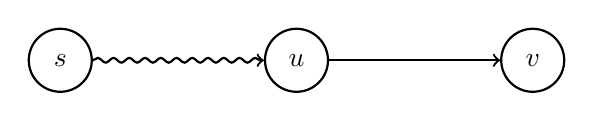
\begin{tikzpicture}[scale=1]
            \node[circle, draw, thick, minimum size=0.8cm] (s) at (0,0) {$s$};
            \node[circle, draw, thick, minimum size=0.8cm] (u) at (3,0) {$u$};
            \node[circle, draw, thick, minimum size=0.8cm] (v) at (6,0) {$v$};

            
            \draw[->, thick, decorate, decoration={snake, amplitude=0.3mm, segment length=2mm}] (s) to[out=0,in=180] (u);
            \draw[->, thick] (u) -- (v);
        \end{tikzpicture}
    \end{figure}

    Отсюда сразу следует, что:
    \begin{equation*}
        \delta_{f_2}(s, v) = \delta_{f_2}(s, u) + 1
    \end{equation*}
    \begin{equation*}
        \delta_{f_2}(s, u) = \delta_{f_2}(s, v) - 1
    \end{equation*}
    
    Заметим, что расстояние до $u$ \textit{не уменьшилось}. Действительно, по определению $v$ -- вершина, которая находится на минимальном расстоянии от $s$. 
    Если бы до $u$ уменьшилось расстояние, то учитывая $\delta_{f_2}(s, v) = \delta_{f_2}(s, u) + 1 > \delta_{f_2}(s, u)$, $u$ -- вершина, которая находилась на ещё меньшем расстоянии, чем $v \Rightarrow$ противоречие.

    Далее пронаблюдаем особенность. Сейчас пойдут интуитивные неформальные рассуждения с амбицией, чтобы читатель понял смысл переходов. У нас была вершина $v$, до которой расстояние уменьшилось и кратчайший путь проходит через вершину $u$, до которой расстояние не уменьшилось, а может даже и увеличилось.
    Эти два факта вместе дают очень интересную мысль: ну если уж до $v$ скоратилось расстояние, то и по идее и до $u$, наверное, оно должно было бы в этом случае сократиться, ведь мы из $u$ напрямую попадаем $v$, пройдя всего по одному ребру и это очень не естественно.
    Кажется довольно логичным исходя из этого предположить, что ребра $(u, v)$ вообще не существовало в $\mathcal{N}_1$. Оказывается, что это правда. Предположим противное, что ребро все же было в $\mathcal{N}_1$. 
    Тогда $\delta_{f_1}(u, v) = 1$, ведь кратчайший путь, который вообще может быть, -- это путь из одного ребра.
    \begin{multline*}
        \delta_{f_1}(s, v) \leq \delta_{f_1}(s, u) + \underbrace{\delta_{f_1}(u, v)}_{1} = \delta_{f_1}(s, u) + 1 \leq \delta_{f_2}(s, u) + 1 = \\
         = \delta_{f_2}(s, v) - 1 + 1 = \delta_{f_2}(s, v)
    \end{multline*}
    \begin{equation*}
        \delta_{f_1}(s, v) \leq \delta_{f_2}(s, v)
    \end{equation*}
    Но, по предположению, до $v$ расстояние уменьшилось, противоречие. Значит, ребра $(u, v)$ изначально в $\mathcal{N}_1$ не было.

    Тогда у нас получается картина такая: в $\mathcal{N}_1$ ребра $(u, v)$ не было, а $\mathcal{N}_2$ оно каким-то образом появилось.
    Такое возможно только, если был \textit{увеличен поток по обратному ребру $(v, u)$}. 
    Напомню, что общая схема была такая: мы идем по увеличивающему пути, потом увеличиваем поток вдоль рёбер, составляющих путь, и одновременно уменьшаем поток в обратных рёбрах.
 
    Теперь вспомним, что ключевая особенность алгоритма Эдмондса-Карпа, которая кажется не особо существенной -- поиск кратчайшего рёберного пути.
    А это значит, что коль скоро мы увеличили поток вдоль ребра $(v, u)$, то в пути $P$, вдоль которого мы увеличивали, $v$ стояло \textit{перед} $u$ (ведь мы прошли именно по ребру $(v, u)$)

    \begin{figure}[h]
        \centering
        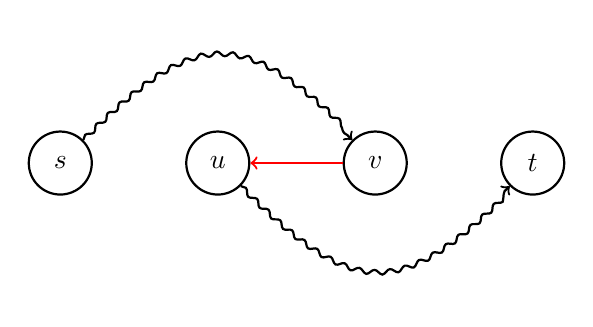
\begin{tikzpicture}[scale=1]
            \node[circle, draw, thick, minimum size=0.8cm] (s) at (0,0) {$s$};
            \node[circle, draw, thick, minimum size=0.8cm] (u) at (2,0) {$u$};
            \node[circle, draw, thick, minimum size=0.8cm] (v) at (4,0) {$v$};
            \node[circle, draw, thick, minimum size=0.8cm] (t) at (6,0) {$t$};

            \draw[->, thick, decorate, decoration={snake, amplitude=0.3mm, segment length=2mm}] 
                (s) to[out=45, in=135, looseness=1.5] (v);
            \draw[->, red, thick] (v) -- (u);

            \draw[->, thick, decorate, decoration={snake, amplitude=0.3mm, segment length=2mm}] 
                (u) to[out=-45, in=-135, looseness=1.5] (t);
        \end{tikzpicture}
    \end{figure}
    Но коль скоро $P$ кратчайший, то все его подпути кратчайшие, а, значит:
    \begin{equation*}
        \delta_{f_1}(s, v) = \delta_{f_1}(s, u) - 1 \leq \underbrace{\delta_{f_2}(s, u)}_{\delta_{f_2}(s, v) + 1} - 1 = \delta_{f_2}(s, v)
    \end{equation*}
    \begin{equation*}
        \delta_{f_1}(s, v) \leq \delta_{f_2}(s, v)
    \end{equation*}
    Получили противоречие с тем, что рёберная длина пути до $v$ уменьшилась. И данное противоречие завершает доказательство.

\end{proof}

\Exe Что если опустить требование к $v$ о минимальности рёберного расстояния? Верны ли будут последующие рассуждения?

\Def Пусть $P$ -- увеличивающий путь. Ребро $e$ пути $P$ будем называть \textit{критическим}, если $c_f(e) = c_f(P)$, где $c_f(P)$ -- пропускная способность пути, определённая на предыдущей лекции.

Далее приведем несколько очевидных утверждений, которые нам понадобятся.

\St Всякий увеличивающий путь имеет хотя бы одно критическое ребро.

\St Если $e$ -- критическое ребро увеличивающего пути $P$, то после очередной итерации алгоритма Эдмондса-Карпа, оно исчезнет из сети.

\Th Число итераций внешнего цикла алгоритма Эдмондса-Карпа равно $\O(|V| |E|)$.
\begin{proof}
    
    Пусть на некоторой итерации алгоритма мы увеличили поток по некоторому увеличивающему пути $P$ в остаточной сети, порожденной потоком $f$. Возьмём произвольное критическое ребро $(u, v)$ пути $P$.

    \begin{figure}[h]
        \centering
        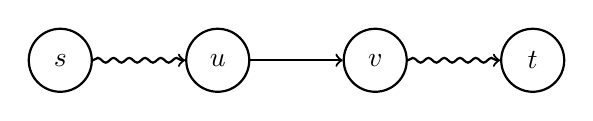
\begin{tikzpicture}[scale=1]
            \node[circle, draw, thick, minimum size=0.8cm] (s) at (0,0) {$s$};
            \node[circle, draw, thick, minimum size=0.8cm] (u) at (2,0) {$u$};
            \node[circle, draw, thick, minimum size=0.8cm] (v) at (4,0) {$v$};
            \node[circle, draw, thick, minimum size=0.8cm] (t) at (6,0) {$t$};

            
            \draw[->, thick, decorate, decoration={snake, amplitude=0.3mm, segment length=2mm}] (s) to[out=0,in=180] (u);
            \draw[->, thick] (u) -- (v);
            \draw[->, thick, decorate, decoration={snake, amplitude=0.3mm, segment length=2mm}] (v) to[out=0,in=180] (t);
        \end{tikzpicture}
    \end{figure}

    Коль скоро путь $P$ кратчайший, то все подпути тоже являются кратчайшими. Следовательно, верно:
    \begin{equation*}
        \delta_f(s, v) = \delta_f(s, u) + 1
    \end{equation*}
    После увеличения потока ребро $(u, v)$ исчезнет из сети, значит, оно точно не будет критическим, как минимум до момента, пока оно снова не появится в ней.
    Но когда исчезвшее ребро может снова появиться? Оно появится, когда мы увеличим поток вдоль обратного ребра -- $(v, u)$. 
    Пусть на некоторой итерации это произошло в сети, порожденной потоком $f'$.

    \begin{figure}[h]
        \centering
        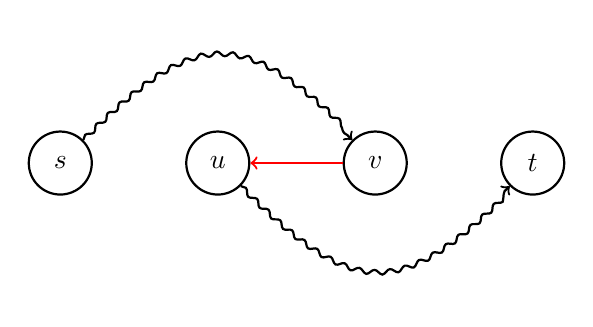
\begin{tikzpicture}[scale=1]
            \node[circle, draw, thick, minimum size=0.8cm] (s) at (0,0) {$s$};
            \node[circle, draw, thick, minimum size=0.8cm] (u) at (2,0) {$u$};
            \node[circle, draw, thick, minimum size=0.8cm] (v) at (4,0) {$v$};
            \node[circle, draw, thick, minimum size=0.8cm] (t) at (6,0) {$t$};

            \draw[->, thick, decorate, decoration={snake, amplitude=0.3mm, segment length=2mm}] 
                (s) to[out=45, in=135, looseness=1.5] (v);
            \draw[->, red, thick] (v) -- (u);

            \draw[->, thick, decorate, decoration={snake, amplitude=0.3mm, segment length=2mm}] 
                (u) to[out=-45, in=-135, looseness=1.5] (t);
        \end{tikzpicture}
    \end{figure}

    Руководствуясь теми же рассуждениями о кратчайших путях:
    \begin{equation*}
        \delta_{f'}(s, u) = \delta_{f'}(s, v) + 1
    \end{equation*}

    Далее, вспоним факт о неубывании расстояния в сети $\Rightarrow \delta_{f'}(s, v) \geq \delta_{f}(s, v)$.
    \begin{equation*}
        \delta_{f'}(s, u) = \delta_{f'}(s, v) + 1 \geq \underbrace{\delta_{f}(s, v)}_{\delta_{f}(s, u) + 1} + 1 = \delta_{f}(s, u) + 1 + 1 = \delta_{f}(s, u) + 2
    \end{equation*}
    \begin{equation*}
        \delta_{f'}(s, u) \geq \delta_{f}(s, u) + 2
    \end{equation*}
    То есть для того, чтобы $(u, v)$ имело хотя бы \textit{возможность} стать критическим (просто существовать в сети), необходимо, чтобы \textit{расстояние от $s$ до $u$ увеличилось хотя бы на $2$}.
    Но какое максимальное расстояние от $s$ до $u$ вообще может быть? Вообще любой простой путь ограничен длиной $|V| - 1$. В <<худшем случае>> у нас возникает путь вида:
    \begin{figure}[h]
        \centering
        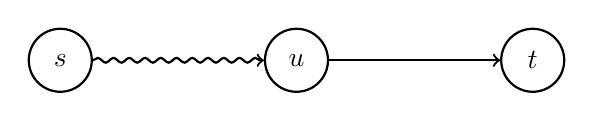
\begin{tikzpicture}[scale=1]
            \node[circle, draw, thick, minimum size=0.8cm] (s) at (0,0) {$s$};
            \node[circle, draw, thick, minimum size=0.8cm] (u) at (3,0) {$u$};
            \node[circle, draw, thick, minimum size=0.8cm] (t) at (6,0) {$t$};

            
            \draw[->, thick, decorate, decoration={snake, amplitude=0.3mm, segment length=2mm}] (s) to[out=0,in=180] (u);
            \draw[->, thick] (u) -- (t);
        \end{tikzpicture}
    \end{figure}

    То есть $u$ стоит прям перед $t$. Значит максимальная длина пути от $s$ до $u$ точно не более $\underbrace{|V| - 1}_{\text{от $s$ до $t$}} - 1 = |V| - 2$ рёбер.

    Коль скоро каждый раз длина пути уменьшается хотя бы на $2$, а максимальная длина не боле $|V| - 2$, то ребро $(u, v)$ станет критическим не более чем $\frac{|V| - 2}{2} = \frac{|V|}{2} - 1$.
    Далее, коль скоро каждый увеличвающий путь состоит хотя бы из одного критического ребра, а также если алгоритм уж кончился, то увеличивающих путей нет, то общее количество итераций алгоритма есть $\O\left(|E| \left( \frac{|V|}{2} - 1 \right) \right) = \O\left(|E| |V| \right)$.

\end{proof}

\Cons Время работы алгоритма Эдмондса-Карпа есть $\O\left(|V| |E|^2\right)$.
\begin{proof}
    
    Каждая итерация цикла работает за $\O(|E|)$, всего итераций $\O(|V| |E|) \Rightarrow$ общее время работы $\O(|V| |E| \cdot |E|) = \O\left(|V| |E|^2\right)$.

\end{proof}
